\chapter{Implementation of domain modeling assistant}

TODO: Brief chapter description.


\section{Generators configuration}

Table (TODO: create table with some prompt examples and add reference) summarizes the configurations of the meta-template for the defined generators. \\

TODO: GitHub prompts directory reference\footnote{\url{https://github.com/Dominik7131/Conceptual-Modeling-LLM-Assistant/tree/master/prompts}}


\subsection{General rules}

We try to design our prompts to resemble LLMs training data to achieve optimal output quality. Given that the majority of this training data is scraped from the internet, we adhere to the following rules:
\begin{itemize}
\item our prompts are only in English
\item unstructured data are inserted in the plain text format
\item structured data are inserted in the JSON format
\end{itemize}


\subsection{Output order}
\label{output_order}
When a human solves the task of generating domain elements solely based on the given domain description he typically proceeds in the following two steps: (1) he finds the context for the given element and (2) from the found context he extracts the specific information such as name of the element.

To mimic this approach, we instruct the LLM in the output specification part to first generate the context for the given element and then to generate the specific information of this element.


\subsection{Output specification}
To improve the response time of our application we instruct the LLM to output one isolated JSON object for each outputted domain element. This way as soon as the LLM generates some proper domain element it can be displayed to the user.


\subsection{Modeling procedure}

TODO: Describe modeling procedure for the classes \\


\subsubsection{Chain of thoughts}

Implementing CoT strategy for generating domain elements is a challenging task as this process does not contain any straightforward steps. As described in the section \ref{output_order} about output order we already instruct the LLM to find the context first and then the specific information.

When instructing the LLM to proceed step by step when generating a domain elements solely based on a given domain description it outputs only the corresponding domain elements in the specified output format.

To put more emphasis on generating the context first of the corresponding domain element, we came up with a simple CoT strategy that instructs the LLM to generate output for each domain element step by step. \\

TODO: Example \\

We propose that other more sophisticated CoT strategies could be used such as when generating attributes to force the LLM to add reason why the outputted object is an attribute. 


\subsection{Tree of thoughts}

TODO: jaký přístup jsme zvolili pro tuto strategii a asi nejdřív to motivovat tím, že naše preliminary experimenty ukázaly, že CoT zlepšuje kvalitu výstupu LLM \\


\subsection{N-shot prompting}

We use examples based on the domain description and its domain model that is shown in the figure \ref{fig:prompting-domain}.

\begin{figure}[!h]
    \centering
    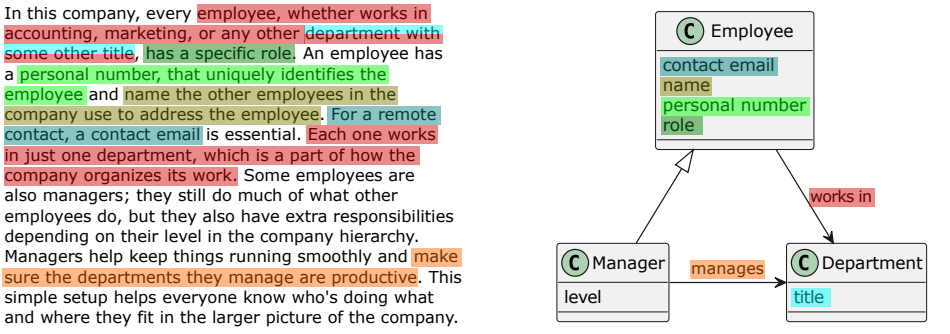
\includegraphics[scale=0.55]{img/prompting-domain.png}
    \caption{\centering The simple company employees domain description and its corresponding domain model used for N-shot prompting in our generator templates}
    \label{fig:prompting-domain}
\end{figure}


For $gen_c$, we use the three classes as examples. For $gen_a$, we use the colored attributes, each with the colored part of the text as examples of the corresponding original texts. For $gen_r$, we proceed similarly, but we provide each sample association twice – for the source class and for the target class.

The concrete examples can be used to further specify the output format. For example,  when the LLM is not provided with a specific name format of the corresponding domain elements, the outputted names can sometimes be in a snake case convention and some other time in a camel case convention. When the provided examples contain a consistent naming format the LLM outputs the provided format consistently. Similarly, this helps to specify the naming style. For example without providing any naming style some generated attributes can contain some unwanted words such as the word ``has'' at the start of the attribute.
